\documentclass{article}

% if you need to pass options to natbib, use, e.g.:
%     \PassOptionsToPackage{numbers, compress}{natbib}
% before loading neurips_2025

% The authors should use one of these tracks.
% Before accepting by the NeurIPS conference, select one of the options below.
% 0. "default" for submission
 \usepackage{neurips_2025}
% the "default" option is equal to the "main" option, which is used for the Main Track with double-blind reviewing.
% 1. "main" option is used for the Main Track
%  \usepackage[main]{neurips_2025}
% 2. "position" option is used for the Position Paper Track
%  \usepackage[position]{neurips_2025}
% 3. "dandb" option is used for the Datasets & Benchmarks Track
 % \usepackage[dandb]{neurips_2025}
% 4. "creativeai" option is used for the Creative AI Track
%  \usepackage[creativeai]{neurips_2025}
% 5. "sglblindworkshop" option is used for the Workshop with single-blind reviewing
 % \usepackage[sglblindworkshop]{neurips_2025}
% 6. "dblblindworkshop" option is used for the Workshop with double-blind reviewing
%  \usepackage[dblblindworkshop]{neurips_2025}

% After being accepted, the authors should add "final" behind the track to compile a camera-ready version.
% 1. Main Track
 % \usepackage[main, final]{neurips_2025}
% 2. Position Paper Track
%  \usepackage[position, final]{neurips_2025}
% 3. Datasets & Benchmarks Track
 % \usepackage[dandb, final]{neurips_2025}
% 4. Creative AI Track
%  \usepackage[creativeai, final]{neurips_2025}
% 5. Workshop with single-blind reviewing
%  \usepackage[sglblindworkshop, final]{neurips_2025}
% 6. Workshop with double-blind reviewing
%  \usepackage[dblblindworkshop, final]{neurips_2025}
% Note. For the workshop paper template, both \title{} and \workshoptitle{} are required, with the former indicating the paper title shown in the title and the latter indicating the workshop title displayed in the footnote.
% For workshops (5., 6.), the authors should add the name of the workshop, "\workshoptitle" command is used to set the workshop title.
% \workshoptitle{WORKSHOP TITLE}

% "preprint" option is used for arXiv or other preprint submissions
 % \usepackage[preprint]{neurips_2025}

% to avoid loading the natbib package, add option nonatbib:
%    \usepackage[nonatbib]{neurips_2025}

\usepackage[utf8]{inputenc} % allow utf-8 input
\usepackage[T1]{fontenc}    % use 8-bit T1 fonts
\usepackage{hyperref}       % hyperlinks
\usepackage{url}            % simple URL typesetting
\usepackage{booktabs}       % professional-quality tables
\usepackage{amsfonts}       % blackboard math symbols
\usepackage{amssymb}        % extended math symbols (\gtrsim, etc.)
\usepackage{nicefrac}       % compact symbols for 1/2, etc.
\usepackage{microtype}      % microtypography
\usepackage{xcolor}         % colors
\usepackage{amsmath}
\usepackage{tikz}
\usetikzlibrary{arrows.meta, positioning, decorations.pathreplacing, calc, patterns}
\usetikzlibrary{positioning, arrows.meta, backgrounds, calc, patterns}
\usepackage{xcolor}
\newcommand{\norm}[1]{\left\lVert#1\right\rVert}


% Note. For the workshop paper template, both \title{} and \workshoptitle{} are required, with the former indicating the paper title shown in the title and the latter indicating the workshop title displayed in the footnote. 
\title{Rethinking Benchmmarking Trajectory Error Accumulation in Fluid Dynamics Datasets}


% The \author macro works with any number of authors. There are two commands
% used to separate the names and addresses of multiple authors: \And and \AND.
%
% Using \And between authors leaves it to LaTeX to determine where to break the
% lines. Using \AND forces a line break at that point. So, if LaTeX puts 3 of 4
% authors names on the first line, and the last on the second line, try using
% \AND instead of \And before the third author name.


\author{%
  ADavid S.~Hippocampus\thanks{Use footnote for providing further information
    about author (webpage, alternative address)---\emph{not} for acknowledging
    funding agencies.} \\
  Department of Computer Science\\
  Cranberry-Lemon University\\
  Pittsburgh, PA 15213 \\
  \texttt{hippo@cs.cranberry-lemon.edu} \\
  % examples of more authors
  % \And
  % Coauthor \\
  % Affiliation \\
  % Address \\
  % \texttt{email} \\
  % \AND
  % Coauthor \\
  % Affiliation \\
  % Address \\
  % \texttt{email} \\
  % \And
  % Coauthor \\
  % Affiliation \\
  % Address \\
  % \texttt{email} \\
  % \And
  % Coauthor \\
  % Affiliation \\
  % Address \\
  % \texttt{email} \\
}


\begin{document}


\maketitle


\begin{abstract}
A recent body of work has developped fully-learned fluid simulators. Methods to train those include single-step training (teacher-forcing), or using unrolled training. For single-step approaches, recent papers have highlighted the importance of capturing high-frequency components to ensure high-fidelity autoregressive rollouts over long horizons.
The question we aim to answer is to what extent each of those approaches relies to the long-term behaviour of the autoregressive rollout. In other terms, we wish to find out what are the main drivers for the drift of a trajectory, and how this differs for existing models. Overall, a formalization of what is the drift and which component are important to reduce it is missing.
\end{abstract}

\section{Introduction}

What leads an autoregressive-model to drift away from a ground-truth trajectory ? What is the role of the single-step prediction in the accumulation of error ? How do such dynamics depend on the dataset in question ? How do different models accumulate different types of errors ? Those are the questions we aim at answering.

\section{Motivation : Why is that important ?}

\begin{itemize}
    \item First of all, to better validate the claimed properties of a new model. For instance, if a model is claimed to better capture the high-frequencies, one should be able to show that the long-term behaviour actually benefits from better captured high-frequencies.
    \item To identify the remaining challenges / parts to improve on a given (dataset, model pair): If the model suffers from exposure bias (going out-of-distribution and performance suffering from this), there should be a specific solution for this. If there is no exposure bias, the one-step prediction and how it emphasizes some frequencies w.r.t others should be the most important part. If it's a conjonction of both, how to address those?
    \item Currently, most works look at: MSE over the rollout / Time of high correlation with the ground-truth, and then validate that the physical consistency is maintained by looking at metrics such as TKE, evolution of the energy spectrum. The latter however don't give a diagnosis on which aspects the model is better than the latter: is is short-term accuracy, no exposure-bias, better captured frequencies ? 
    \item To know what to expect from a model on a new dataset, as well as for reproducibility: by looking only at the MSE of the model, a new practicionner/researcher doesn't know how a model should behave/easier debugging
\end{itemize}

\section{Background : ML-based Fluid Simulators}

\section{Sources of error amplification in autoregressive models}

\subsection{Definitions : One-Step error, Systematic-Drift and Exposure-Bias}

We assume access to a neural-operator $NO$, which given only access to an initial condition $x_0$, aims at predicting the subsequent states $\{\hat{x}_1, ..., \hat{x}_K\}$ that closely match the ground-truth trajectory $\{x_1, ..., x_K\}$, in an autoregressive manner : 
\begin{align}
    \hat{x}_1 &= NN(x_0)\\
    \forall t \in \{2, ..., K\} \ \ \hat{x}_t &= NN(\hat{x}_{t-1})
\end{align}
Given the initial data distribution $p_0$, we define the pushforward data distributions $p_t$, $t=1,...,K$
\begin{align}
    X_t = GT(X_{t-1}), \ X_{t} \sim p_t, X_{t-1} \sim p_{t-1}
\end{align}

corresponding to the data distribution after $t$ ground-truth simulation steps.

At a given timestep $t$, we write
\begin{align}
    \hat{X}_t = NN(\hat{X}_t) = X^{ID}_t + \epsilon^{OOD}_t
\end{align} where $X^{ID}_t$ is the sample in $p_t$ that lies the closest (according to some metric to be defined) to $\hat{X}_t$. We then decompose the error $\epsilon(t) = \norm{\hat{X}_t - X_t} = \norm{NN^{(t)}}$ as :

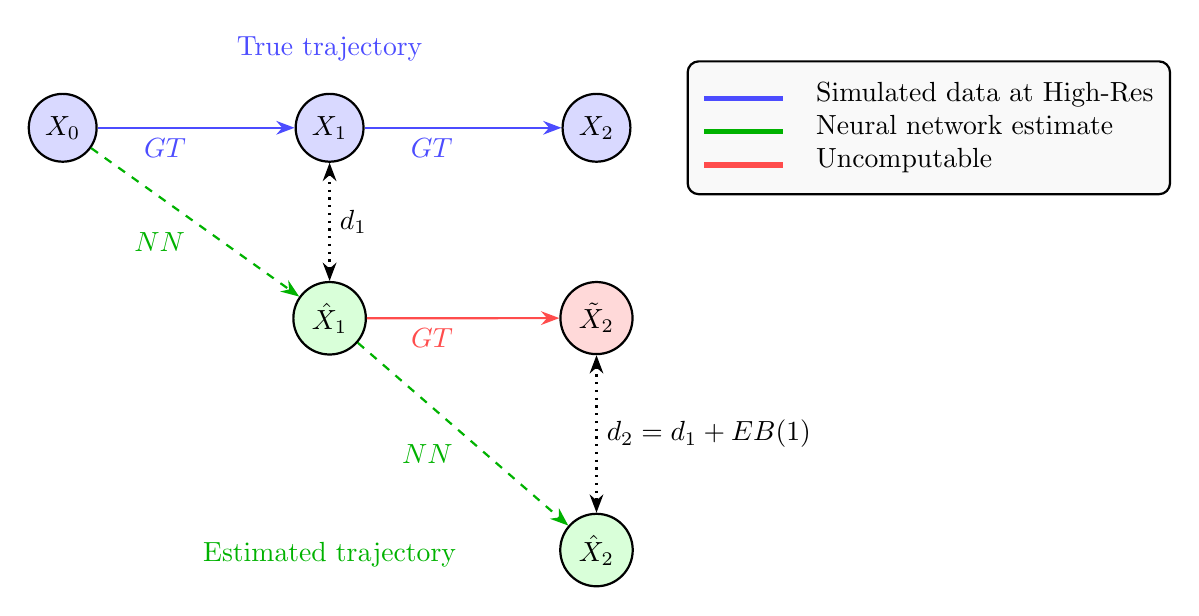
\begin{tikzpicture}[>=Stealth, node distance=2.5cm, thick]

% Define nodes
\node[circle, draw, fill=blue!15] (X0) {$X_0$};
\node[circle, draw, fill=blue!15, right=of X0] (X1) {$X_1$};
\node[circle, draw, fill=blue!15, right=of X1] (X2) {$X_2$};

\node[circle, draw, fill=green!15, below=1.5cm of X1] (Xh1) {$\hat{X}_1$};
\node[circle, draw, fill=red!15, below=1.5cm of X2] (Xh2GT) {$\tilde{X}_2$};
\node[circle, draw, fill=green!15, below=2cm of Xh2GT] (Xh2) {$\hat{X}_2$};

% Draw arrows for the true trajectory
\draw[->, thick, blue!70] (X0) -- node[pos=0.5, below left] {$GT$} (X1);
\draw[->, thick, blue!70] (X1) -- node[pos=0.5, below left] {$GT$} (X2);

% Draw arrows for the estimated trajectory
\draw[->, thick, green!70!black, dashed] (X0) -- node[pos=0.5, below left] {$NN$} (Xh1);
\draw[->, thick, green!70!black, dashed] (Xh1) -- node[pos=0.5, below left] {$NN$} (Xh2);

% Draw arrow for the uncomputable (red) connection
\draw[->, thick, red!70] (Xh1) -- node[pos=0.5, below left] {$GT$} (Xh2GT);

% --- NEW: dotted double arrows with labels d1 and d2 ---
\draw[<->, thick, dotted] (X1) -- node[right] {$d_1$} (Xh1);
\draw[<->, thick, dotted] (Xh2GT) -- node[right] {$d_2 = d_1 + EB(1)$} (Xh2);

% Labels
\node[blue!70, above of=X1, node distance=1cm] {True trajectory};
\node[green!70!black, below of=Xh1, node distance=3cm] {Estimated trajectory};

% ------------------------------------------------------------------
% Color legend box
% ------------------------------------------------------------------
\begin{scope}[shift={(11, 0)}] % adjust position as needed
  \node[draw, rounded corners, fill=gray!5, inner sep=6pt] (legend) {
    \begin{tabular}{@{}ll@{}}
      \textcolor{blue!70}{\rule{1cm}{2pt}} & Simulated data at High-Res \\
      \textcolor{green!70!black}{\rule{1cm}{2pt}} & Neural network estimate \\
      \textcolor{red!70}{\rule{1cm}{2pt}} & Uncomputable \\
    \end{tabular}
  };
\end{scope}

\end{tikzpicture}

\begin{figure}

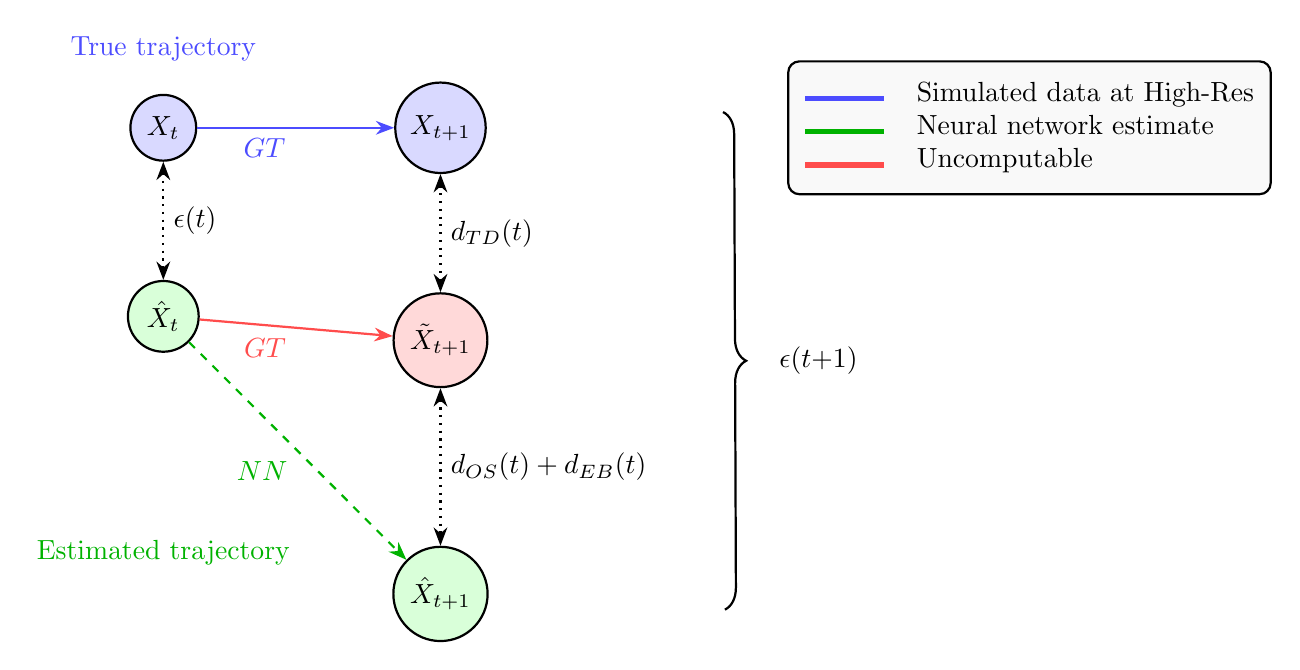
\begin{tikzpicture}[>=Stealth, node distance=2.5cm, thick]

% Define nodes
\node[circle, draw, fill=blue!15] (X1) {$X_t$};
\node[circle, draw, fill=blue!15, right=of X1] (X2) {$X_{t+1}$};

\node[circle, draw, fill=green!15, below=1.5cm of X1] (Xh1) {$\hat{X}_t$};
\node[circle, draw, fill=red!15, below=1.5cm of X2] (Xh2GT) {$\tilde{X}_{t+1}$};
\node[circle, draw, fill=green!15, below=2cm of Xh2GT] (Xh2) {$\hat{X}_{t+1}$};

% True trajectory
\draw[->, thick, blue!70] (X1) -- node[pos=0.5, below left] {$GT$} (X2);

% Estimated trajectory
\draw[->, thick, green!70!black, dashed] (Xh1) -- node[pos=0.5, below left] {$NN$} (Xh2);

% Uncomputable link
\draw[->, thick, red!70] (Xh1) -- node[pos=0.5, below left] {$GT$} (Xh2GT);

% Dotted double arrows
\draw[<->, thick, dotted] (X2) -- node[right] {$d_{TD}(t)$} (Xh2GT);
\draw[<->, thick, dotted] (X1) -- node[right] {$\epsilon(t)$} (Xh1);
\draw[<->, thick, dotted] (Xh2GT) -- node[right] {$d_{OS}(t) + d_{EB}(t)$} (Xh2);

% --- NEW: Brace from X_{t+1} to \hat{X}_{t+1} ---
\draw[decorate, decoration={brace, amplitude=8pt}, thick]
  ($(X2.east)+(3,0.2)$) -- ($(Xh2.east)+(3,-0.2)$)
  node[midway, xshift=1.2cm] {$\epsilon(t{+}1)$};

% Labels
\node[blue!70, above of=X1, node distance=1cm] {True trajectory};
\node[green!70!black, below of=Xh1, node distance=3cm] {Estimated trajectory};

% ------------------------------------------------------------------
% Color legend box
% ------------------------------------------------------------------
\begin{scope}[shift={(11, 0)}]
  \node[draw, rounded corners, fill=gray!5, inner sep=6pt] (legend) {
    \begin{tabular}{@{}ll@{}}
      \textcolor{blue!70}{\rule{1cm}{2pt}} & Simulated data at High-Res \\
      \textcolor{green!70!black}{\rule{1cm}{2pt}} & Neural network estimate \\
      \textcolor{red!70}{\rule{1cm}{2pt}} & Uncomputable \\
    \end{tabular}
  };
\end{scope}

\end{tikzpicture}
\label{fig:decomposition}
\caption{Decomposition into Systematic Drift, One-Step Error, and Exposure-Bias}
\end{figure}

We have that :

\begin{align*}
    \norm{\hat{X}_{t+1} - X_{t+1}} = \epsilon(t+1) &\leq \norm{X_{t+1} - \tilde{X}_{t+1}} + \norm{\tilde{X}_{t+1} - \hat{X}_{t+1}} \\ 
    &\leq \textcolor{blue}{\norm{X_{t+1} - {\tilde{X}_{t+1}}}} + \textcolor{green}{\norm{GT(\hat{X}_{t}) - NN\left(\hat{X}_t^{ID}\right)}} + \textcolor{red}{\norm{NN\left(\hat{X}_t^{ID}\right) - NN\left(\hat{X}_t\right)}} \\
    &= \textcolor{blue}{d_{TD}(t)} + \textcolor{green}{d_{OS}(t)} + \textcolor{red}{d_{EB}(t)}
\end{align*}
where each term represents, respectively:
\begin{itemize}
    \item The \textit{Trajectory-Drift} error $d_{TD}(t)$ resulting from the accumulation of errors from earlier steps, and which only depends on emulator calls up to $t-1$.
    \item The \textit{One-Step} error $d_{OS}(t)$ which is the systematic error incurred at every step. If we assume that the ground-truth distribution stays constant during the simulation, i.e. $p_t = p_{t-1}$, we can write $d_{OS}(t) = d_{OS}$
    \item The \textit{Exposure-Bias} error $d_{EB}(t)$ which is the additional error due to the discrepancy between $\hat{p}_t$ and $p_t$.
\end{itemize}
Note that after a single simulation step, since the input to the model is the in-distribution groundtruth $x_0$, the error only contains one-step error: $\norm{\hat{X}_1 - X_1} = d_{OS}(0)$.

\subsection{Identifying the contribution of each factor}

For a given model and dataset, we aim at giving a characterization of the sources of error in order to design taylored improvements. However, there are two issues:
\begin{itemize}
    \item In general one only has access to a high-resolution simulator $GT^{high}$, therefore evaluations of $GT$ on arbitrary generated points $\hat{X}_{t+1}$ are inaccessible.
    \item It is not clear how to compute the in-distribution equivalent $\hat{X}_t^{ID}$
\end{itemize}

We argue that typically reported metrics, such as overall MSE over a trajectory or high-correlation time, don't give enough information on the reasons why a model drifts, and are not satisfactory, especially for long rollouts where random effects can largely influence the generated trajectory.

Furthermore, we argue that for each dataset, the main driver of drift w.r.t the ground-truth trajectory can be vastly different. We use this to motivate the fact that, models developed for a given task (such as PDERefiner for KolmogorovFlow and Kuramoto-Sivashinsky, which are inherently small one-step error dependent, are not suitable for datasets where the main error driver is exposure bias and systematic drift, such as Transonic Flow). 

\subsection{Obtaining a proxy for the model Ground-truth prediction}


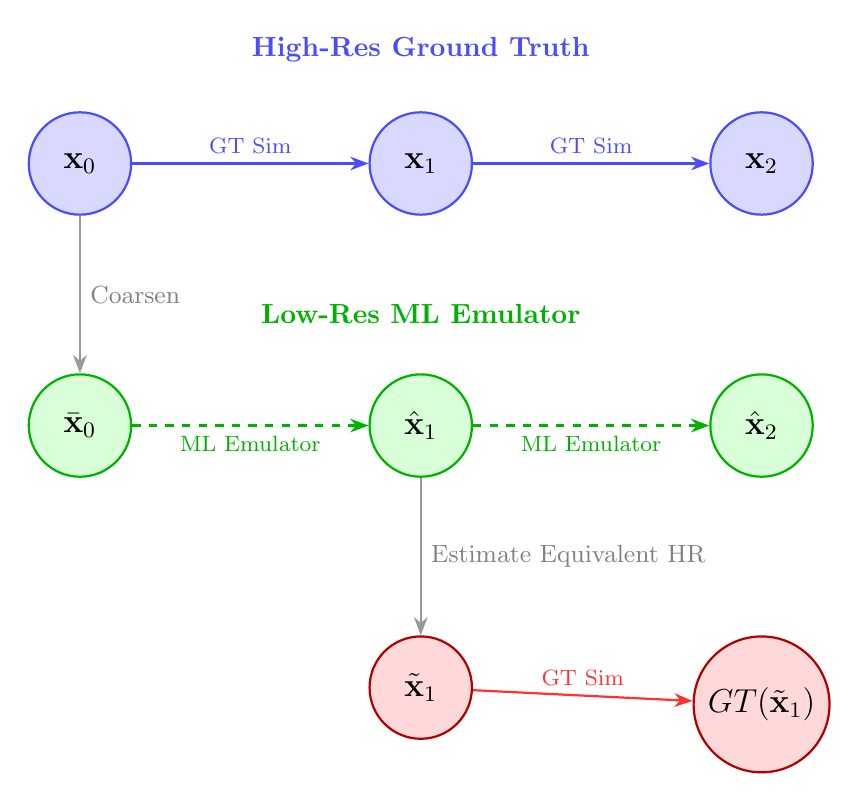
\begin{tikzpicture}[>=Stealth, node distance=3cm, thick]

% --- Style Definitions based on input example ---
% HR Nodes (Blueish)
\tikzstyle{hr_node}=[circle, draw=blue!70, thick, fill=blue!15, minimum size=1.3cm, font=\large]
% LR Nodes (Greenish)
\tikzstyle{lr_node}=[circle, draw=green!70!black, thick, fill=green!15, minimum size=1.3cm, font=\large]
% Proxy HR Nodes (Redish)
\tikzstyle{proxy_hr_node}=[circle, draw=red!70!black, thick, fill=red!15, minimum size=1.3cm, font=\large]

% Arrow Styles
\tikzstyle{gt_arrow}=[->, thick, blue!70]
\tikzstyle{ml_arrow}=[->, thick, green!70!black, dashed]
\tikzstyle{coarsen_arrow}=[->, thick, gray!80]
\tikzstyle{proxy_gt_arrow}=[->, thick, red!80]


% --- Define Nodes ---

% Time t=0
\node[hr_node] (X0_HR) {$\mathbf{x}_0$};
% The LR start is a coarsened version of the HR start, placed below it
\node[lr_node, below=2cm of X0_HR] (X0_LR) {$\bar{\mathbf{x}}_0$};

% Time t=1
\node[hr_node, right=of X0_HR] (X1_HR) {$\mathbf{x}_1$};
\node[lr_node, right=of X0_LR] (X1_LR) {$\hat{\mathbf{x}}_1$};
\node[proxy_hr_node, below=2cm of X1_LR] (X1_PHR) {$\tilde{\mathbf{x}}_1$};

% Time t=2
\node[hr_node, right=of X1_HR] (X2_HR) {$\mathbf{x}_2$};
\node[lr_node, right=of X1_LR] (X2_LR) {$\hat{\mathbf{x}}_2$};
\node[proxy_hr_node, below=2cm of X2_LR] (X2_PHR) {$GT(\tilde{\mathbf{x}}_1)$};

% --- Draw Connections ---

% 1. The initial coarsening step
\draw[coarsen_arrow] (X0_HR) -- node[right, font=\small, color=gray] {Coarsen} (X0_LR);

% 2. The HR Ground Truth Trajectory (Solid Blue)
\draw[gt_arrow] (X0_HR) -- node[midway, above, font=\footnotesize] {GT Sim} (X1_HR);
\draw[gt_arrow] (X1_HR) -- node[midway, above, font=\footnotesize] {GT Sim} (X2_HR);

% 3. The LR ML Emulator Trajectory (Dashed Green)
\draw[ml_arrow] (X0_LR) -- node[midway, below, font=\footnotesize] {ML Emulator} (X1_LR);
\draw[ml_arrow] (X1_LR) -- node[midway, below, font=\footnotesize] {ML Emulator} (X2_LR);

%4 . The LR to Proxy HR
\draw[coarsen_arrow] (X1_LR) -- node[right, font=\small, color=gray] {Estimate Equivalent HR} (X1_PHR);

%4 . The Proxy HR to next Proxy HR
\draw[proxy_gt_arrow] (X1_PHR) -- node[midway, above, font=\footnotesize] {GT Sim} (X2_PHR);


% --- Labels for the Trajectories ---
\node[blue!70, above=0.5cm of X1_HR, font=\bfseries] {High-Res Ground Truth};
\node[green!70!black, above=0.5cm of X1_LR, font=\bfseries] {Low-Res ML Emulator};


\end{tikzpicture}

The estimate $\tilde{\mathbf{x}}_1$ must be very precise, in order for the GT transition to be accurate. A super-resolution operation based only on $\hat{\mathbf{x}}_1$ is intuitively not sufficient. Therefore, our approach consists in optimizing the initial condition of a chain of high-resolution simulations to make the final coarsened state match the low-resolution model prediction.

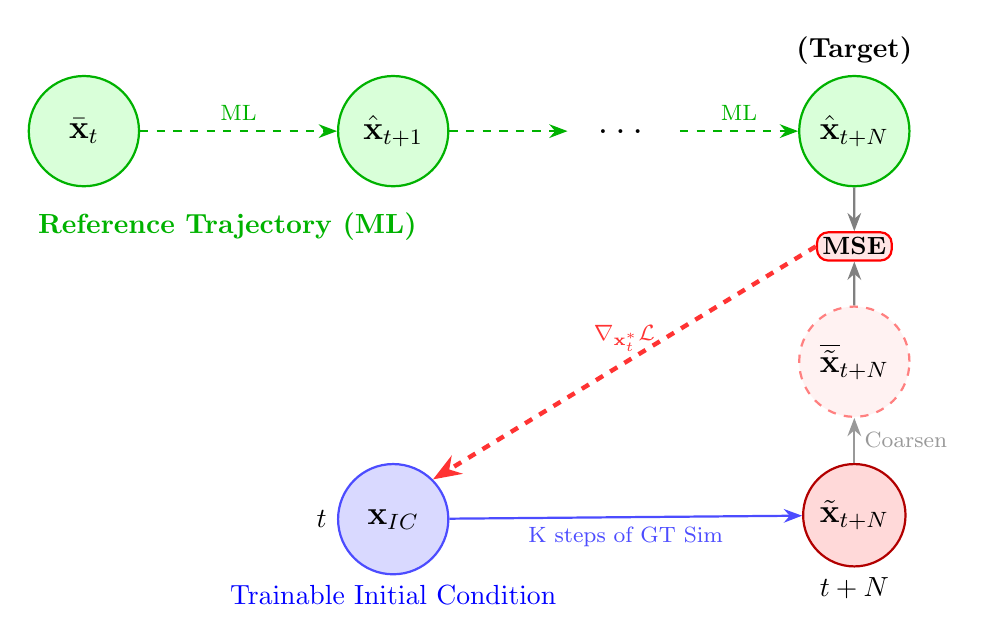
\begin{tikzpicture}[>=Stealth, node distance=2.5cm, thick]

% --- Style Definitions ---
% HR Nodes (Blueish)
\tikzstyle{hr_node}=[circle, draw=blue!70, thick, fill=blue!15, minimum size=1.4cm, font=\large]
% LR Nodes (Greenish)
\tikzstyle{lr_node}=[circle, draw=green!70!black, thick, fill=green!15, minimum size=1.4cm, font=\large]
% Ellipsis Node (Invisible box for spacing)
\tikzstyle{dots_node}=[minimum size=1.4cm, font=\bfseries\Large]
% Loss Node
\tikzstyle{loss_node}=[rectangle, rounded corners, draw=red, fill=red!10, thick, inner sep=2pt, font=\small\bfseries]
\tikzstyle{proxy_hr_node}=[circle, draw=red!70!black, thick, fill=red!15, minimum size=1.3cm, font=\large]

% Arrow Styles
\tikzstyle{gt_arrow}=[->, thick, blue!70]
\tikzstyle{ml_arrow}=[->, thick, green!70!black, dashed]
\tikzstyle{coarsen_arrow}=[->, thick, gray!80]
\tikzstyle{grad_arrow}=[->, ultra thick, red!80, dashed]


% --- 1. Top Row: ML Emulator (Target) ---

% Start (t)
\node[lr_node, label=] (ML_0) {$\bar{\mathbf{x}}_t$};
% Next (t+1)
\node[lr_node, right=of ML_0] (ML_1) {$\hat{\mathbf{x}}_{t+1}$};
% Ellipsis
\node[dots_node, right=1.5cm of ML_1] (ML_dots) {$\dots$};
% End (t+N)
\node[lr_node, right=1.5cm of ML_dots, label=\textbf{(Target)}] (ML_N) {$\hat{\mathbf{x}}_{t+N}$};

% Draw ML Path
\draw[ml_arrow] (ML_0) -- node[midway, above, font=\footnotesize] {ML} (ML_1);
\draw[ml_arrow] (ML_1) -- (ML_dots);
\draw[ml_arrow] (ML_dots) -- node[midway, above, font=\footnotesize] {ML} (ML_N);


% --- 2. Bottom Row: Physics Optimization Loop ---

% Trainable Input (t)
\node[hr_node, below=3.5cm of ML_1, label={below:\textcolor{blue}{Trainable Initial Condition}}, label={left:$t$}] (Opt_0) {$\mathbf{x}_{IC}$};
\node[proxy_hr_node, below=3.5cm of ML_N, label={below:$t+N$}] (Opt_N) {$\tilde{\mathbf{x}}_{t+N}$};

% Draw GT Path
\draw[gt_arrow] (Opt_0) -- node[midway, below, font=\footnotesize] {K steps of GT Sim} (Opt_N);


% --- 3. The Comparison Step (End) ---

% Coarsen the final physics state
\node[lr_node, dashed, draw=red!50, fill=red!5, below=1.5cm of ML_N] (Opt_N_Coarse) {$\overline{\tilde{\mathbf{x}}}_{t+N}$};

% Arrow from HR final to Coarse final
\draw[coarsen_arrow] (Opt_N) -- node[right, font=\footnotesize] {Coarsen} (Opt_N_Coarse);

% Loss Calculation
\node[loss_node] (Loss) at ($(ML_N)!0.5!(Opt_N_Coarse)$) {MSE};

% Connect Target and Prediction to Loss
\draw[->, gray, thick] (ML_N) -- (Loss);
\draw[->, gray, thick] (Opt_N_Coarse) -- (Loss);


% --- 4. Gradient Flow (Backpropagation) ---

% Draw a big sweeping arrow from Loss back to Opt_0
% We navigate around the "dots" to make it look clean

\draw[grad_arrow] (Loss.west) -- node[midway, above, font=\footnotesize] {$\nabla_{\mathbf{x}_t^*} \mathcal{L}$} (Opt_0.north east);


% --- Annotations & Legend ---

\node[anchor=west, text=green!70!black, font=\bfseries] at (ML_0.west |- ML_0.south) [yshift=-0.5cm] {Reference Trajectory (ML)};


\end{tikzpicture}

Using more GT Sim calls leads to a more physically-plausible state (it acts as a regularizer, i.e. after only a few simulator calls, the output may still contain non-physical artifacts), but it's also more expansive, and potentially harder to optimize. Also since the problem is under-determined (the target is a low-resolution field for which there may be infinitely-many relevant high-resolution fields). There regularization terms could also be explored to constrain the space of high-resolution states.

The main issue of this method is that it is slow: it runs backpropagation operations at high-resolution. It is furthermore required to run this optimization for every datapoint, and every autoregressive call. It also requires a high amount of GPU RAM (already 30 GB for batch-size of 5 and 2 simulator calls)... If one only uses this approach post-training as an analysis tool, this is probably fine. 

As an alternative to retraining an initial condition for every (data index, AR step) pair, one could train a neural network to map the initial condition to the refined one (this would be less memory expansive, at the expense of being accurate). Note that in this problem we actually want to overfit, since we want to exactly match the model's predicted state.


\section{The trajectory drift}

Assuming that we can write the 

The trajectory drift is influenced by the "shape" of the error. In other words, starting from a same initial condition $X_t$, two trajectories from two different neural operators $\hat{X}_{t+1}^{(1)}$ and $\hat{X}_{t+1}^{(2)}$ with a same one-step eror $\left(d_{OS}^{(1)}(t) = d_{OS}^{(2)}(t)\right)$, may have a different next-step trajectory drift : $d_{TD}^{(1)}(t+1) \neq d_{TD}^{(2)}(t+1)$. This is because a given trajectory may diverge faster from the ground-truth trajectory depending on which errors are made compared to that trajectory.

\subsection{The Pareto-front of frequency errors : Highlighting the trajectory drift effect}

Assuming that a neural emulator has a fixed one-step error, and no exposure bias. We aim at identifying the response of the trajectory drift to the shape of the one-step error. Since we once again don't have access to a ground-truth simulator to which one could inject an error of a given shape, we make use of two neural emulators, and look at the linear combination between them.

We look at applying transformations to the two model's predictions


\section{Finding the optimal trade-off between Exposure-Bias and Performance} 

As mentioned, it is not sufficient to look at training process error, as it could lead to exposure bias.
Furthermore, it is also not sufficient to look at the sampling process error, as the reduction of error in a given timestep may come from reduction in other timesteps. Our aim is to isolate the effect that a given timestep will incur in the next timesteps, as exposure bias. in previous timesteps directly impact error in current timestep.

We highlight a few points:
\begin{itemize}
    \item if a model has exposure bias then it is likely that 
    \item How close the input error needs to be 
    \item How much of the "exposure-bias" comes from the fact that the model is not supposed to be deterministic ? Rather than drifting ? 
\end{itemize}

\subsubsection{Model Cross-Comparisons : A proxy metric for exposure bias}

The intuition is the following: Given the trajectory $\{\hat{x}_1, .., \hat{x}_K\}$ obtained from autoregressive sampling of $NO_1$, if both models have a low exposure bias, then the average distance between $\hat{x}_t$ and $NO_2(\hat{x}_{t-1})$ should not vary much as a function of $t$. 
Note that this is only a sufficient condition: if the average distance between $NO_1$ and $NO_2$ stays constant, it doesn't imply that they are both exposure-bias free.

By using multiple "reference" (evaluation) models, we can (potentially?) get rid of the case where the distance between models doesn't increase with constant distance. We may also be able to obtain a more accurate estimate of each model's biases.

In particular, we look at the evolution of: 
\begin{align}
    \mathbb{E} \lVert \hat{x}_t - NO_2(\hat{x}_{t-1}) \rVert^2 &= \mathbb{E} [ \epsilon(x_t)^2  + \lVert NO_2(\hat{x}_{t-1}) - GT(\hat{x}_{t-1}) \rVert^2 \\ &  \ \ \ \ - 2 \langle\hat{x}_t  - GT(\hat{x}_{t-1}), NO_2(\hat{x}_{t-1}) - GT(\hat{x}_{t-1})\rangle ] \\
    &= \mathbb{E}\left[\left(\epsilon_{NN_1}(x_0) + EB_{NN_1}(\hat{x}_{t-1}\right)^2\right]
\end{align}
The second term is the single-step error made by the second neural-operator. It can also be decomposed as a sum of the systematic drift of $NO_2$, and the exposure-bias of $NO_2$ when using the trajectory of $NO_1$ as input.

\textbf{In practice}, we observe that a cross-correlation doesn't necessarily induce a faster increase of error. The reason could be two things:
\begin{itemize}
    \item The cross-correlation is not a good indicator of the exposure bias ? Indeed, the cross-correlation implies that the samples generated by the neural emulator become out-of-distribution. It however doesn't necessarily imply that the model suffers from this drift. Still, is it possible that two models get further from each other and their performance does not degrade ? Can we think about 2-steps metric to show that a model indeed suffers from its own drift ? Like Eval(M1(M1(x))) vs M1(M1(x)) (regarde carnet).
    \item If use one model to evaluate, could just mean that it is more sensible to a certain type of drift than another. Can either : evaluate with more models. Actually, the cross-comparison of a diffusion model with a certain schedule and a diffusion model with another schedule is non-increasing (it even decreases). 
    \item The cross-correlation is a good indicator of the exposure bias, but exposure bias becomes insignificant in the error accumulation (due for instance, to dynamics). In particular, at the time where exposure bias is too high, the trajectory has maybe drifted so much that the error cannot be seen.
    \item How to explain that evaluating a diffusion model traj. with a diffusion model evaluator leads to a reduction of error as a function of the simulation step ? 
    \item The evaluator is the one that suffers from the out-of-distribution : the discrepancy at a given timestep could hinder the evaluator rather than the model itself.
\end{itemize}

\subsection{Ideas of cross-comparisons evaluations}

\begin{itemize}
    \item On the trajectory of $M_1$, apply $M_2$ (with less exposure bias, for instance a 2-steps Unet which has no out-of-distribution samples). We assume that this will "put back" the sample more in-distribution. Then apply $M_1$ again, and compare to applying $M_1$ twice. 
\end{itemize}


\subsection{The exposure bias of different neural emulators}

\section{Experiment log}

\subsection{Phases of the project}

\paragraph{PHASE 1: Identify how HR proxy emulation works}

- Are there any troubles with it
- What are the metrics of interest to measure how good the estimate is
- What is the correct way to initialize the initial condition (before optimization) :
    - initial condition may influence how easy it is to obtain a correct or incorrect solution to the optimization problem
- Explore how the dataset influences the correctness of the estimate, w.r.t the defined metrics
- Effect of the hyperparameters (number of proxy simulator calls, number of optimization steps, type of input at initialization, regularization of the prediction)

\textbf{There, the main point is ensuring the unconditional (dataset and model independent) correctness of the proxy estimator. If the proxy is incorrect, the downstream uses of it are useless}

\paragraph{PHASE 2: Exploring the potential downstream applications of the HR proxy emulation}

\subsection{Logs}

\paragraph{13.02.2026}
An important issue seems to be the computational overhead required to optimize the initial condition in high-resolution. For a batch size of 4, and 15 AR steps, 1000 steps of optimization take more than 10 hours. The question is whether we can juggle with the parameters (increasing model calls and decreasing number of steps) to cope with that. The issue is that we will anyway not be able to run the experiment on a batch of 64, let alone the full validation set. 

$\rightarrow$ Attempt to cope with that : look at effect of number of optimization steps on accuracy at ts.1. Explore the NB STEPS x MODEL CALLS GRID

Result : for Kolmo, 5 calls seems to be a good starting point. Also, lower learning rate (0.001) leads to less explosion. 

\paragraph{14.02.2026}
Obtaining results on a single trajectory, for Diffusion Adaptive UT :
\begin{figure}[h]
  \centering
  \includegraphics[width=0.95\textwidth]{/mnt/SSD2/constantin/drift-bench/outputs/2026-02-14/00-09-48/proxy_gt_metrics.png}
  \label{fig:140226}
\end{figure}

It's not sure whether the increase is due to :
\begin{itemize}
  \item (1) Harder optimization at later steps
  \item (2) Harder One-step error depending on position on trajectory
  \item (3) Actual Exposure-Bias
\end{itemize}
(1) The type of initialization "model-traj" is good for steps larger than n simulator calls, but for earlier steps it still uses the GT traj, which could lead to unequal treatment. (2) Adding the Proxy GT vs Model on Proxy GT Error as a proxy should get rid of point. This sould give a closer baseline, if the one-step error fluctuates based on the position in the trajectory. 

Overall, a guarantee of the correctness of the Proxy is very important. 

\paragraph{15.02.2026}
Now with the Proxy GT vs Model on Proxy GT:
\begin{figure}[h]
  \centering
  \includegraphics[width=0.95\textwidth]{/mnt/SSD2/constantin/drift-bench/outputs/2026-02-14/13-44-11/proxy_gt_metrics.png}
  \label{fig:150226}
\end{figure}

The two curves follow each other closely, showing the fluctuations are due to the fluctuations in the trajectory rather than in exposure-bias / estimate correctness. This at least shows that the proxy is able to consistently (in the same way) match the model trajectory (for timesteps $\geq$ 2).

We see an increase in the ratio between the two curves at timestep 2, and then close to no increase (at eye view).

The question is whether this increase is due to exposure-bias, or due to bad calibration/convergence of the proxy. Also, could just be that the distance is due to the fact that there is no high-resolution proxy which can match the low-resolution model prediction.

\textbf{Might not be able to give a certificate, but at least can we put the initial prediction in "disadvantage", i.e. make initial condition further away from trajectory}

\paragraph{16.02.2026}

Meeting with Felix. Advices: start with 1D cases where we don't actually need to run a coarsening operation.  Simple cases would also allow to have a better characterization of what it means to be "in-distribution" (Fourier approach). Furthermore, one can iterate faster (his advice is : simulation should take in order of seconds, training should take in order of 10 minutes).

This makes sure that we have full vision (for instance, in the HR case, we only compare the LR fields, so the HR potentially could be out-of-dist). Multi-resolution could be a next step.

So start with advection, KS even, Burgers. Or chaotic case where we can validate that drifting obeys to chaos theory. 

The plan is therefore to start with exponax, compute the initial condition for a lot of trajectories, get the exposure-bias. Maybe we can also get a characterization of the error separation.

\paragraph{18.02.2026}
First runs on APEBench, 1D Advection, checking the different training options (one, sup unrolling, diverted chain unrolling), with advection gamma equal to 10.5

On this case, multiple questions:
- one has a better first-step mse than sup;2 and sup;5, which is intuitive
- however, one has a worse first-step mse than div;2 and div;5, which is not intuitive (check myself what div means, and ask Felix if doesn't make sense still)
- we also see that among one, sup;2 and sup;5, sup;5 has worse first-step MSE, but best long-term MSE, which is intuitive. Question is whether this difference is due to exposure-bias reduction, or to predictive placement.

I think that, without diving into Exposure-Bias etc, the first hypothesis is that first-step MSE does a big part of the job. This sounds obvious, but this is probably a finding to display. In the sense that now, when creating a new architecture/model, one should display which part of the trajectory improves. Check which proporition of the PDEs is defined by the one-step MSE, 

There is also the hypothesis made in APEBench that unrolling could increasing the receptive field and therefore lead to better one-step prediction ? Not sure though. It's also claimed that the diverted training is a good trade-off between one-step MSE and long-term performance. Indeed, that's the case. Using that method is therefore a matter of what's important for a given design in mind. 

Ran experiments on FNO: 

\begin{figure}[h]
  \centering
  \includegraphics[width=0.95\textwidth]{/mnt/SSD2/constantin/drift-bench/outputs/2026-02-14/13-44-11/proxy_gt_metrics.png}
  \label{fig:180226_fno}
\end{figure}

My hypothesis is that the only thing that architectures modify is the one-step MSE, in most cases. Especially, when training them in one-step, architectures in general have the same error growth. Actually, that's not true for all architectures (and a regularization method can be thought of as being part of the architecture, for instance adding noise on input in diffusion models as in ACDM), but in most cases it is true. The question is rather, can we categorize architectures into categories of brougth improvements. for instance that training with noiThey don't bring an 


Idea for the diffusion project: 
What about using different models, maybe also during inference. Could also vary the architectures, if it turns out that an architecture is better for a given noise range. This would increase the model size by 3 or 4, but in a smart way. And if we can show it improves the performance better than a classical ensemble, would be nice. 

But for now, let's say we want a single model: we can train a model fully on the lowest noise level, actually just pick the one with the lowest sampling error (rather than taking a parameter tau). Then we train earlier step, using binary search. And iterate. Or we train it all at the same time, and

\section{Discussions with Claude}

\subsection{Frequency distribution of one-step error and its effect on rollout}

A natural question is whether two models with the same total one-step MSE but different spectral error profiles will exhibit different rollout behaviour. By Parseval's theorem, the MSE decomposes exactly into per-mode contributions:
\begin{align}
    \norm{\hat{x} - x}^2 = \sum_k |\hat{\tilde{x}}_k - \tilde{x}_k|^2
\end{align}
so at the single-step level, MSE is frequency-agnostic: an error of magnitude $\epsilon$ at wavenumber $k_1$ contributes identically to an error of the same magnitude at wavenumber $k_2$.

However, the picture changes drastically when we consider autoregressive rollout. The key observation is that the \textit{trajectory drift} $d_{TD}(t)$ depends not only on the magnitude of the one-step error, but on its spectral distribution.

\paragraph{The general case: forward energy cascade.} In most 3D turbulent systems, energy cascades from large scales to small scales (forward cascade). In such systems:
\begin{itemize}
    \item \textbf{Low-frequency errors} corrupt the large-scale structure of the flow. Since the large scales govern advection and the overall trajectory of the system, these errors propagate to all scales through nonlinear mode coupling. A wrong large-scale flow transports features to wrong locations, leading to rapid trajectory divergence.
    \item \textbf{High-frequency errors} are noise-like and tend to be damped by physical dissipation (viscosity). They remain spectrally localized for short times and have a weaker feedback onto the large-scale dynamics.
\end{itemize}

Therefore, a model whose one-step error is concentrated in low frequencies will typically exhibit faster trajectory drift than one whose error is concentrated in high frequencies, even at equal total MSE. This favours architectures like UNets, whose spatial locality and pooling hierarchy naturally capture low-frequency structure well, even if they smear high-frequency detail.

\paragraph{The inverse cascade case: Kolmogorov flow.} Kolmogorov flow is 2D Navier-Stokes with sinusoidal forcing at a fixed wavenumber, and is one of the most common benchmarks in the neural operator literature. Crucially, 2D turbulence exhibits an \textit{inverse energy cascade}: energy injected at small scales flows upward to larger scales, while enstrophy cascades downward.

In this regime, the argument reverses. High-frequency errors can feed energy upward into the large-scale structure through the inverse cascade, eventually corrupting it. Getting the small scales right therefore matters for the large-scale trajectory, which means the FNO's purported advantage at high frequencies could genuinely translate into better rollout stability on this specific benchmark.

Other systems exhibiting inverse cascades include rotating and stratified (geophysical) flows, thin fluid films, and certain MHD configurations.

\paragraph{Role of the Reynolds number.} The Reynolds number $\text{Re} = UL/\nu$ controls the ratio of inertial to viscous forces and determines the width of the inertial range over which the cascade operates.
\begin{itemize}
    \item At \textbf{low Re} (typical of many benchmarks, $\text{Re} \sim 100$--$1000$), viscosity damps fluctuations efficiently across scales. The inverse cascade has limited room to operate, and errors at small scales are dissipated before they can migrate significantly upward. The spectral distribution of error has a moderate effect on rollout.
    \item At \textbf{high Re} ($\text{Re} \gtrsim 10000$), the inertial range is wide and the inverse cascade is vigorous. High-frequency errors have many scales to climb through and can seriously corrupt large-scale structures during rollout.
\end{itemize}

This means that model comparisons are Reynolds-number dependent: a UNet and an FNO may show similar rollout behaviour at moderate Re, while at high Re the difference in their spectral error profiles becomes decisive. This should be taken into account when designing benchmarks and interpreting results: the Re at which a benchmark is run determines how much the spectral structure of the one-step error matters for long-term trajectory fidelity.

\paragraph{Implications for benchmarking.} This analysis suggests that reporting only aggregate one-step MSE (or even rollout MSE) is insufficient. One should additionally report:
\begin{itemize}
    \item The spectral decomposition of the one-step error (per-wavenumber MSE)
    \item The Reynolds number and cascade regime of the benchmark system
    \item Whether rollout improvements stem from better low-frequency or high-frequency accuracy
\end{itemize}
This would allow distinguishing whether a claimed architectural improvement (e.g., ``better high-frequency capture'') actually benefits the downstream rollout task, or whether it merely redistributes error across frequencies without affecting trajectory drift.

\paragraph{A 1D test case: Kuramoto-Sivashinsky.} The frequency-dependent rollout effect can also be observed in 1D, using the Kuramoto-Sivashinsky (KS) equation. The KS equation features a linear instability band at intermediate wavenumbers that injects energy, while the quadratic nonlinearity $u \cdot u_x$ redistributes energy across scales. Crucially, this redistribution goes \textit{both directions}: forward to high wavenumbers (where the hyperdiffusion $u_{xxxx}$ dissipates it) and backward to low wavenumbers. This partial inverse transfer means that high-frequency errors can feed into low-$k$ modes through nonlinear interactions.

The linear growth rate per wavenumber $k$ is:
\begin{align}
    \sigma(k) = \underbrace{|\gamma_2| \, k^2}_{\text{anti-diffusion (energy injection)}} - \underbrace{|\gamma_4| \, k^4}_{\text{hyper-diffusion (dissipation)}}
\end{align}
Modes are linearly unstable where $\sigma(k) > 0$, i.e.\ for $k < k_c$ where:
\begin{align}
    k_c = \sqrt{\frac{|\gamma_2|}{|\gamma_4|}}
\end{align}
With default parameters ($\gamma_2 = -1.2$, $\gamma_4 = -15.0$), this gives $k_c \approx 0.28$. To widen the instability band so that the task relies more on high-frequency accuracy, one increases the ratio $|\gamma_2|/|\gamma_4|$, pushing $k_c$ to higher wavenumbers.

Additionally, the KS equation is chaotic (positive Lyapunov exponents), so any perturbation grows exponentially. However, the rate of growth depends on which modes are perturbed: errors in the linearly unstable band (the most dynamically active wavenumbers) are amplified fastest.

This makes KS a suitable 1D testbed for the spectral error experiment: given two models with the same total one-step MSE, one with error concentrated at low-$k$ and one at high-$k$, we expect different rollout divergence rates. The chaotic dynamics should amplify the difference, and the partial inverse transfer should make high-frequency errors more consequential than in a purely forward-cascade system.

By contrast, Burgers' equation is less informative for this analysis: it is not chaotic (shocks are attracting structures), so errors are either absorbed into shocks or advected away rather than cascading across scales.

\paragraph{10.03.2026} The issue with the approach is that the proxy GT is not able to match well the ML simulator trajectory, and the error is much lower for $t=0$ than for even $t=1$. For $t>1$, it appears the error between the proxy GT and the ML simulation is stable for unrolled steps. See top right plot, which shows error between ML trajectory, and proxy step, for $K=1$. Behaviour is similar for larger $K$.

\begin{figure}
   \centering
  \includegraphics[width=0.95\textwidth]{/mnt/SSD2/constantin/drift-bench/outputs/2026-03-10/proxy_model_evaluation.pdf}
  \label{fig:100326_proxy}
\end{figure}

Actually, let's try to not compare the model's prediction with the GT on the GT proxy, as it may be arbitrary far away. What we want to know is whether a ML model suffers from its own distribution more than it would suffer from a GT state. By suffering, we therefore mean that its error is further away from the GT trajectory (total trajectory error). Therefore, at each step in the ML trajectory, we can run the ML model on the proxy GT, the ML model on itself, and compute the 2 errors w.r.t the GT trajectory.
Also one must compute the difference in 
 error between $MSE(NN(x_hat), x_gt)$ and $MSE(NN(x_tilde, x_gt))$ to ensure that the cost of out-of-dist input is not just due to the proxy gt being     
closer to the true trajectory.

\begin{figure}
   \centering
  \includegraphics[width=0.95\textwidth]{/mnt/SSD2/constantin/drift-bench/outputs/2026-03-10/nn_on_own_traj_vs_nn_on_proxy_gt.pdf}
  \label{fig:100326_proxy}
\end{figure}

\paragraph{10.03.2026 - 2}

In previous figure, it appears there is a difference in error between calling NN on its own traj, vs calling it on the GT traj, however, there is also a difference in the original error (spatial advantage). I don't think it's a relevant metric to compare to the true GT because it quickly accumulates too much.

An alternative is: at a given step $t$, compute the GT proxy. Then for a given $s$, run $s$ GT steps from there, and look at the error betwen $\hat{x}_{t+k}$ and $GT^k(\tilde{x})$. Look at how this error evolves with time. We expect that a model suffers from its out-of-distribution if the error increases. Since the proxy estimate's error, as seen above, doesn't increase as $t$ increases, it's likely that the metric is accurate.

\begin{figure}
   \centering
  \includegraphics[width=0.95\textwidth]{/mnt/SSD2/constantin/drift-bench/outputs/2026-03-10/proxy_gt_called_multiple_times_time_evolution.pdf}
  \label{fig:100326_proxy}
\end{figure}

\paragraph{10.03.2026 - 3}

We need more than just a trend. We need a precise characterization of each term. We want to know: at a given timestep, what is the contribution of each term, as in Figure \ref{fig:decomposition}. First, we need to check if the sum of the three terms actually reaches the full trajectory error at a given step. This would be a first point to know if the characterization can be done.

\paragraph{11.03.2026}

In order for the decomposition to be useful, we need to either show that it's exact, or at least show that it's able to rank different models in the same order as they are ranked in terms of the trajectory drift, at each timestep. If the models are not ranked similarly, then the metric isn't useful.

\end{document}
